\documentclass{TDP005mall}
\usepackage{graphicx}


\newcommand{\version}{Version 1.0}
\author{Elliot Johansson, \url{elljo130@student.liu.se}\\
  Lukas Freyland, \url{lukfr510@student.liu.se}\\
  Nadim Lakrouz, \url{nadla777@student.liu.se}}
\title{Designspecifikation}
\date{2022-11-25}
\rhead{Elliot Johansson\\
Lukas Freyland\\
Nadim Lakrouz}



\begin{document}
\projectpage
\section{Revisionshistorik}
\begin{table}[!h]
\begin{tabularx}{\linewidth}{|l|X|l|}
\hline
Ver. & Revisionsbeskrivning & Datum \\\hline

1.0 & Första utkast & 2022-11-25 \\\hline
\end{tabularx}
\end{table}

\section{Player}

Syftet med Playerklassen är att representera den karaktär spelaren styr. Spelaren styr vilka formler playerkaraktären använder. Spelaren kommer inte förflytta sig på planen. Vissa formler kommer behöva riktas för att träffa fienderna medan andra inte behöver det.
Funktionen regenerate\_mana kommer sakta återställa manapoäng med sf:Clock.

\subsection{}

\begin{itemize}
    \item int hp - privat variabel som tilldelas ett heltal. 
    \item double mana - privat variabel som tilldelas ett flyttal. 
    \item sf:Clock clock - sfml variabel för att hantera tiden.
    \item int set\_hp() - ändrar privata variabeln hp.
    \item int get\_hp() - hämtar privata variabeln hp.
    \item int get\_mana() - hämtar privata variabeln mana.
    \item void regenerate\_mana() - ökar privata variabeln mana över tid.
   
\end{itemize}


\section{Enemies}
''Enemies'' klassens syfte är att representera fienderna som i intervaller kommer förflytta sig mot spelaren på spelplanen. Enemies har en check\_collision funktion som anropas när fiender och spelare kolliderar.
\subsection{}

\begin{itemize}

    \item double hp - privat variabel som tilldelas ett flyttal. 
    \item double resistance - privat variabel som tilldelas ett flyttal.
    \item void check\_collision() - kollar kollision med spelaren och magiska formler. 
    \item int set\_hp() - ändrar privata variabeln hp.
    \item int get\_hp() - hämtar privata variabeln hp.
    \item int get\_resistance() - hämtar privata variabeln resistancce.
    \item void ai\_movement() - styr fiende rörelse. 
    
\end{itemize}

\section{Spells\_Handler}

\begin{itemize}

    \item pair<string, int> mana\_per\_spell - lista med hur mycket mana varje magiska formel kostar. 
    \item void handle\_input() - hanterar spelarens inmätning. 
    \item void handle\_combination() - hanterar kombinationer av magiska     formler. 
    \item void handle\_damage() - beräknar och hanterar damage. 
    \item void control\_spell() - navigerar spells med hjälp av mus. 
    
\end{itemize}

\section{Diagram}
\begin{center}
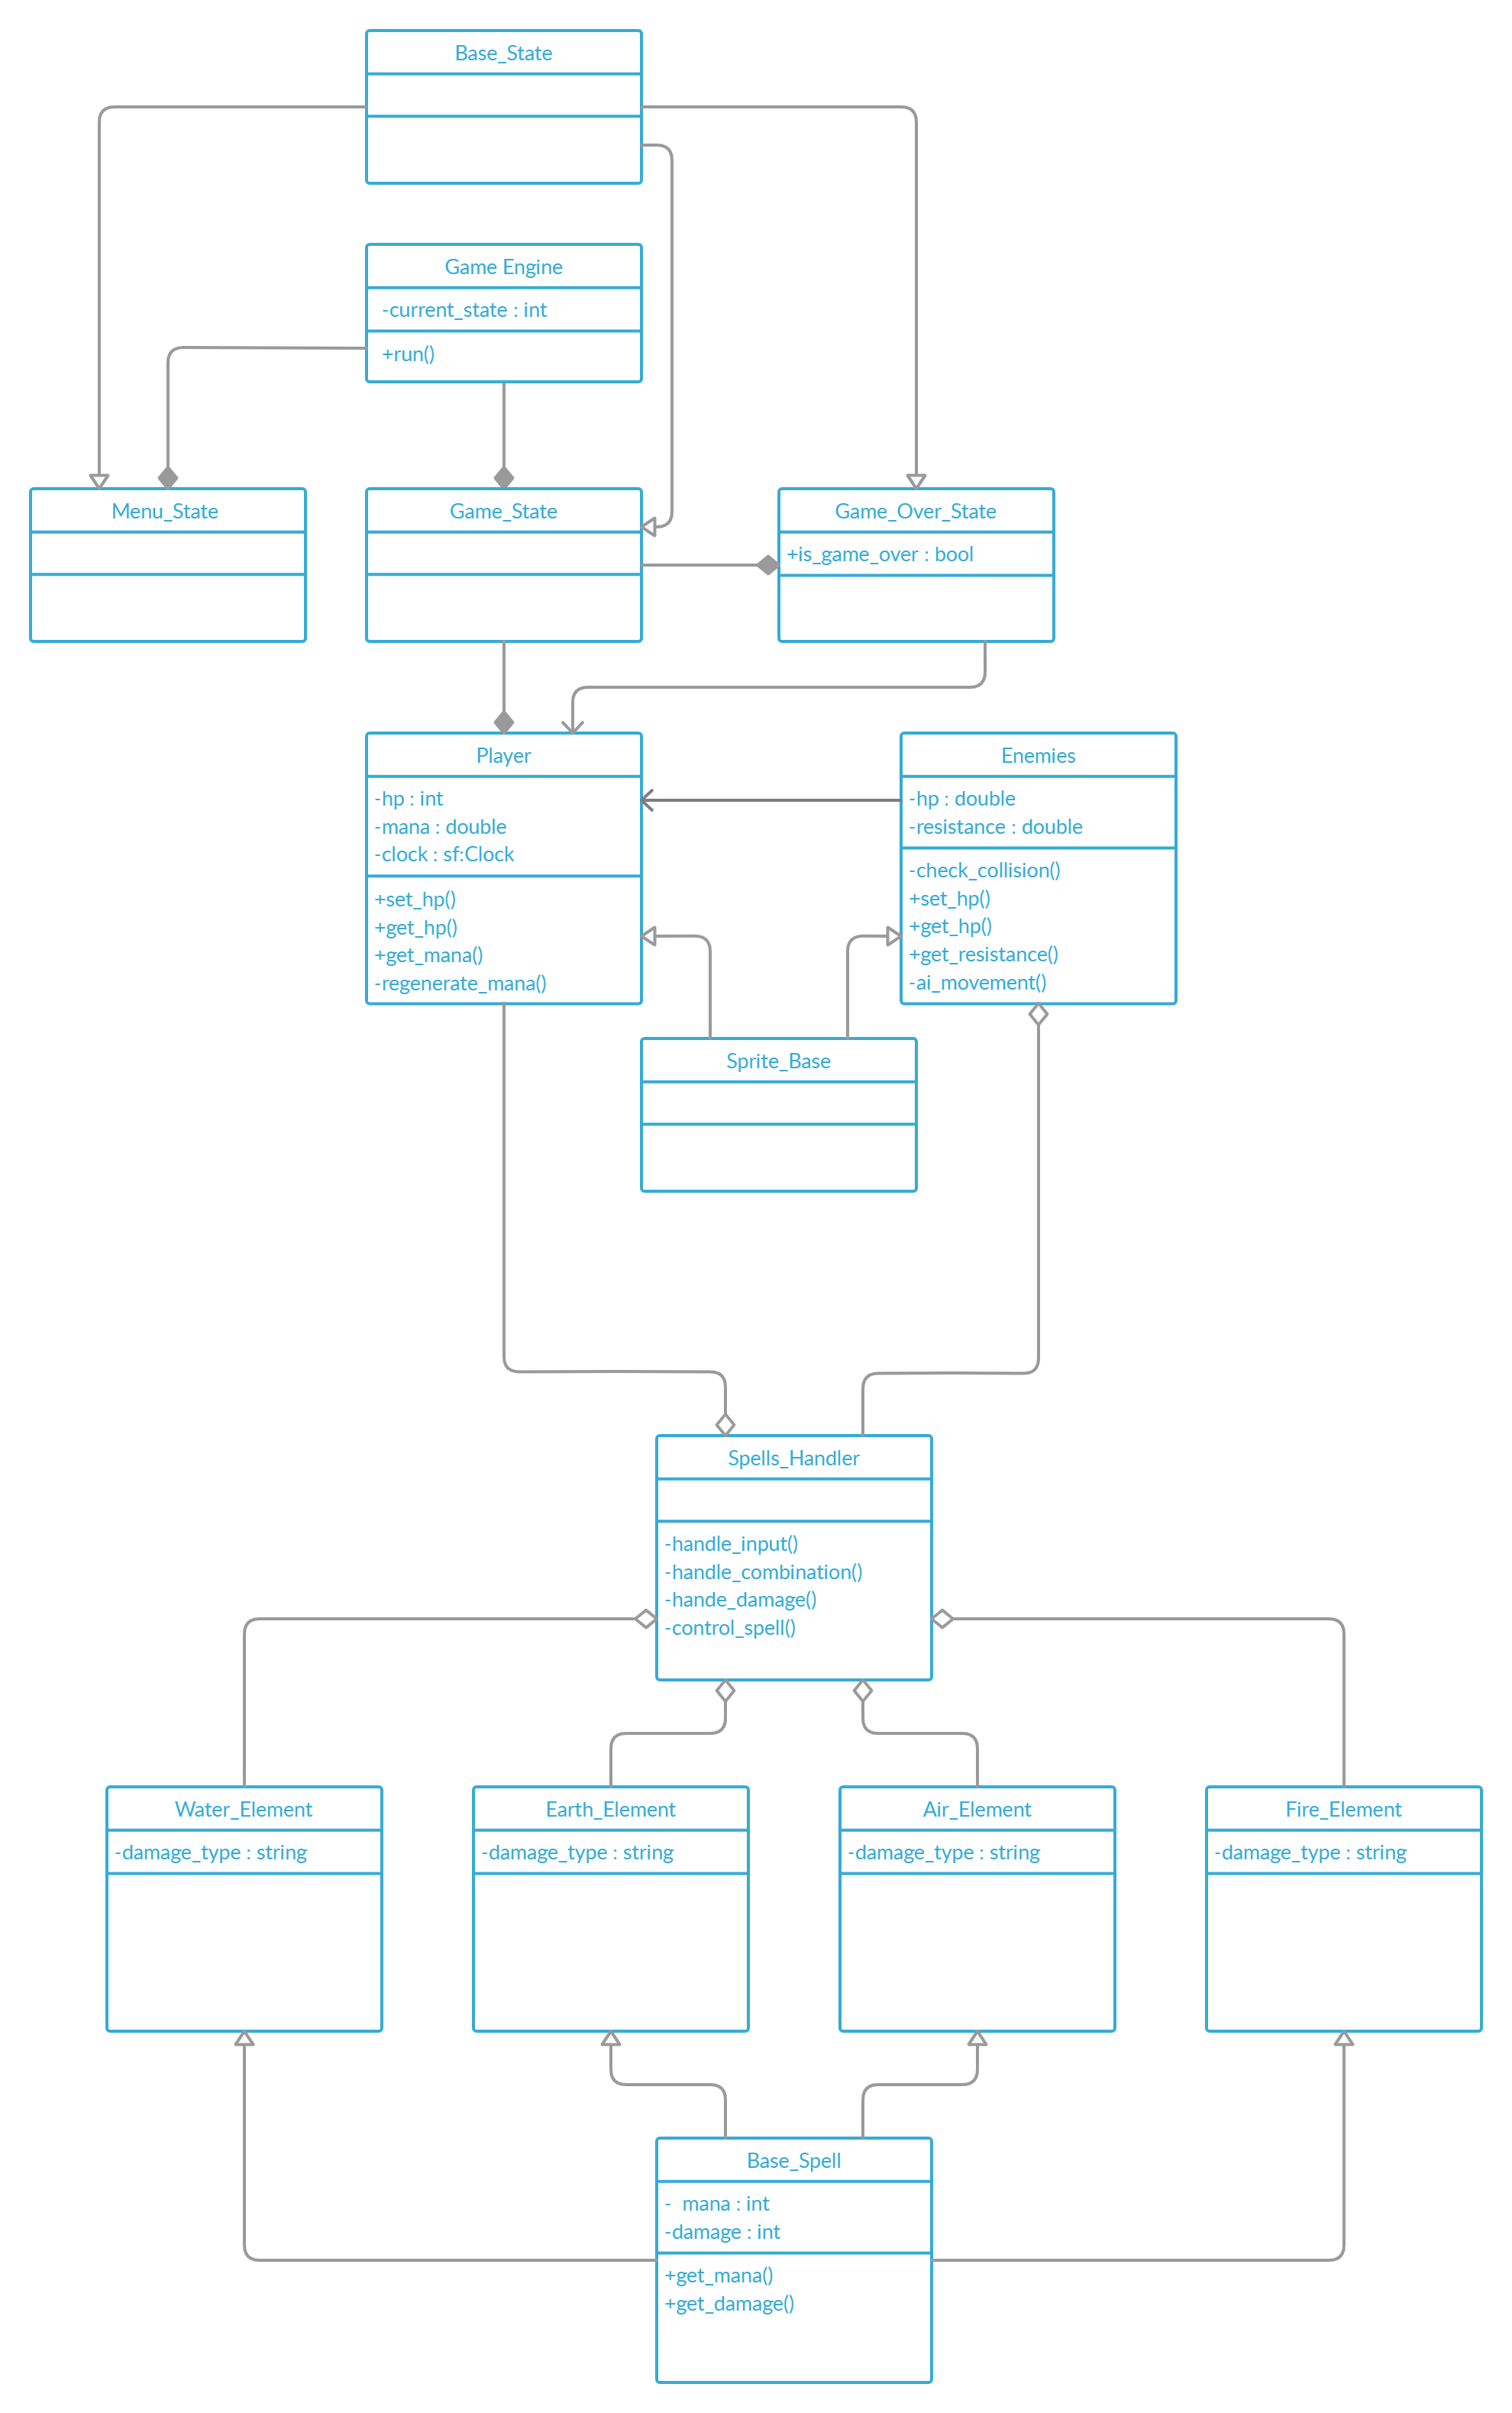
\includegraphics[scale=0.18]{uml_diagram.jpg}
\end{center}
\end{document}
